\documentclass[conference]{IEEEtran}

% \IEEEoverridecommandlockouts
% The preceding line is only needed to identify funding in the first footnote. If that is unneeded, please comment it out.

% %%%%%%%%%%%%%%%%%%%%%%%%%%%%%%%%%%%%%%%%%%%%%%%%%%%%%%%%%%%%%%%%%%%%%%%%%%%%%
% Packages
% %%%%%%%%%%%%%%%%%%%%%%%%%%%%%%%%%%%%%%%%%%%%%%%%%%%%%%%%%%%%%%%%%%%%%%%%%%%%%

\usepackage{cite}
\usepackage{amsmath,amssymb,amsfonts}
\usepackage{algorithmic}
\usepackage{graphicx}
\usepackage{textcomp}
\usepackage{xcolor}
\usepackage{booktabs}
\usepackage{listings}
\usepackage{pgfplots}
\lstdefinestyle{column-code}{
    language=C++,                                     % choose the language of the code
    basicstyle=\scriptsize\ttfamily,basewidth=0.75em, % the size of the fonts that are used for the code
    numbers=left,                   % where to put the line-numbers
    numberstyle=\scriptsize,        % the size of the fonts that are used for the line-numbers
    stepnumber=1,                   % the step between two line-numbers. If it is 1 each line will be numbered
    numbersep=5pt,                  % how far the line-numbers are from the code
    backgroundcolor=\color{white},  % choose the background color. You must add \usepackage{color}
    showspaces=false,               % show spaces adding particular underscores
    showstringspaces=false,         % underline spaces within strings
    showtabs=false,                 % show tabs within strings adding particular underscores
    frame=single,                   % adds a frame around the code
    tabsize=2,                      % sets default tabsize to 3 spaces
    captionpos=b,                   % sets the caption-position to bottom
    breaklines=true,                % sets automatic line breaking
    breakatwhitespace=false,        % sets if automatic breaks should only happen at whitespace
    linewidth=\columnwidth,
    boxpos=b,
    xleftmargin=2em,
    framexleftmargin=1.5em,
    %escapeinside={\%
    %}
    %{
    %)}          % if you want to add a comment within your code
}

\lstdefinestyle{full-code}{
    language=C++,                                     % choose the language of the code
    basicstyle=\scriptsize\ttfamily,basewidth=0.75em, % the size of the fonts that are used for the code
    numbers=left,                   % where to put the line-numbers
    numberstyle=\scriptsize,        % the size of the fonts that are used for the line-numbers
    stepnumber=1,                   % the step between two line-numbers. If it is 1 each line will be numbered
    numbersep=5pt,                  % how far the line-numbers are from the code
    backgroundcolor=\color{white},  % choose the background color. You must add \usepackage{color}
    showspaces=false,               % show spaces adding particular underscores
    showstringspaces=false,         % underline spaces within strings
    showtabs=false,                 % show tabs within strings adding particular underscores
    frame=single,                   % adds a frame around the code
    tabsize=2,                      % sets default tabsize to 3 spaces
    captionpos=b,                   % sets the caption-position to bottom
    breaklines=true,                % sets automatic line breaking
    breakatwhitespace=false,        % sets if automatic breaks should only happen at whitespace
    linewidth=\textwidth,
    boxpos=b,
    xleftmargin=2em,
    framexleftmargin=1.5em,
    %escapeinside={\%
    %}
    %{
    %)}          % if you want to add a comment within your code
}

\renewcommand{\lstlistingname}{Code}

\def\BibTeX{{\rm B\kern-.05em{\sc i\kern-.025em b}\kern-.08em
    T\kern-.1667em\lower.7ex\hbox{E}\kern-.125emX}}

% %%%%%%%%%%%%%%%%%%%%%%%%%%%%%%%%%%%%%%%%%%%%%%%%%%%%%%%%%%%%%%%%%%%%%%%%%%%%%
% Begin Document
% %%%%%%%%%%%%%%%%%%%%%%%%%%%%%%%%%%%%%%%%%%%%%%%%%%%%%%%%%%%%%%%%%%%%%%%%%%%%%

\begin{document}

% %%%%%%%%%%%%%%%%%%%%%%%%%%%%%%%%%%%%%%%%%%%%%%%%%%%%%%%%%%%%%%%%%%%%%%%%%%%%%
% Title
% %%%%%%%%%%%%%%%%%%%%%%%%%%%%%%%%%%%%%%%%%%%%%%%%%%%%%%%%%%%%%%%%%%%%%%%%%%%%%

\title{Spectrum: Classifying, Replicating and Mitigating Spectre Attacks on a Speculating RISC-V Microarchitecture}

% %%%%%%%%%%%%%%%%%%%%%%%%%%%%%%%%%%%%%%%%%%%%%%%%%%%%%%%%%%%%%%%%%%%%%%%%%%%%%
% Authors
% %%%%%%%%%%%%%%%%%%%%%%%%%%%%%%%%%%%%%%%%%%%%%%%%%%%%%%%%%%%%%%%%%%%%%%%%%%%%%

\author{\IEEEauthorblockN{Gonzalez, Abraham}
\IEEEauthorblockA{\textit{CS 262A}\\ \textit{CS 294-156}} \\
\and
\IEEEauthorblockN{Korpan, Ben}
\IEEEauthorblockA{\textit{CS 262A}\\ \textit{CS 294-156}} \\
\and
\IEEEauthorblockN{Younis, Ed}
\IEEEauthorblockA{\textit{CS 262A}\\ \textit{CS 261}} \\
\and
\IEEEauthorblockN{Zhao, Jerry}
\IEEEauthorblockA{\textit{CS 294-156}} \\
}

\maketitle

\begin{abstract}
    %TODO: does the last sentence sound good

    The discovery of exploits targeting the effects of speculative execution has
    forced the computer architecture community to rethink the design space of
    high-performance and secure microarchitectures. This new category of attacks,
    broadly categorized as ``Spectre'', has spurred substantial research on how to
    mitigate vulnerabilities associated with high-performance microarchitectural
    features. In this paper, we present three results to advance research on
    secure hardware mitigations for these threats; a taxonomy for speculative style
    attacks and defenses, replication of speculative attacks on an open-source processor,
    and a hardware implementation of a speculative buffer cache that mitigates
    basic speculative cache attacks.
    
    We have categorized the variety of attacks based on if the attacks are 
    architecturally legal and the defenses based on their types. Additionally, 
    we have mapped mitigations to the attacks that they potentially cover.
    Using the Berkeley Out-Of-Order Machine (BOOM), we have 
    re-implemented Spectre Variants 1 and 2 that target the L1 Data Cache. We 
    achieve a leakage rate of around 114 bytes per sec with a 100 MHz processor 
    frequency. Additionally, we propose and implement a speculative buffer,
    called SpecBuf, that holds speculative data in the MSHRs until commit where the 
    data will be transfered to the L1. Based on preliminary results, it achieves 
    a 2216 Dhrystones/s score on the Dhrystone benchmark
    resulting in a 2\% performance increase compared to the
    baseline. Additionally, trial synthesis on a 45nm process shows a 2.5\% area
    increase and 0.36\% clock reduction. To our knowledge, these replications and 
    SpecBuf implementation is the first demonstration of a speculative style attack
    on BOOM and the first synthesizable RTL implementation of a speculative buffer.
\end{abstract}

\section{Introduction}

Ever since the disclosure of Spectre and Meltdown at the start of 2018, there has
been a large number of attacks targeting speculative microarchitectural state in
out-of-order processors \cite{b1,b2}. Each of these attacks is able to exploit the shared
state of the processor between a victim process/thread and a malicious process/thread.
While classifications have been developed for cache-based and for timing-based 
side-channel attacks \cite{b5,b6,b7,b9,b10}, a general taxonomy for these attacks has not been adopted.
A well-devised taxonomy would inform not only the 
categorization of new attacks but also the development of hardware mitigations for 
these attacks. A complete categorization system would help hardware researchers 
identify general mitigations for broad categories of vulnerabilities, instead of 
targeted fixes for specific attacks.

Additionally, the Berkeley Out-of-Order Machine (BOOM) open-source RISC-V
microarchitecture has yet not been exposed to these types of attacks \cite{b11}. BOOM
is a generic implementation of a speculative 
out-of-order microarchitecture that employs many of the same features as the 
out-of-order systems targeted by published attacks. Generic, open-source 
implementations of attacks and their mitigation strategies would provide a common 
foundation for the development of defenses for speculative execution attacks.
By attacking an open-source machine with Spectre, researchers can not only gain more 
insight into the malicious attack but also attempt to mitigate the attack on a shared,
open platform. Moreover, this project hopes to unify and guide the attack 
mitigation process. With an attack taxonomy and an open-source microarchitecture, a 
newly proposed mitigation technique can easily target a class of attacks as informed 
by the taxonomy.

The remainder of this paper is structured as follows: In Section 2, we discuss
related works that indicate relevant work that introduces attacks, defenses, and classifications.
In Section 3 we discuss our taxonomy and it's categorization of the attacks and defenses. In
Section 4 we present the subset of attacks that were replicated for this paper. In Section 5
we discuss the implementation of the SpecBuf. In Section 6 we discuss the evaluation of the
replications and the SpecBuf. In Section 7 we discuss future work.

\section{Related Works}

\subsection{Speculative Style Attacks}

\subsubsection{Spectre}

This work first described a speculative style attack on out-of-order cores that 
allows a malicious user to read secret data from a victim \cite{b1}. When an out-of-order 
processor reaches a control flow instruction, it uses the Branch Target Buffer in 
conjunction with the Branch Predictor to make an educated guess on the direction
of program flow. If the control flow is mispredicted then the code that was
executed will not be committed into the architectural state. However, the
speculated instruction can changed the microarchitectural state causing data
leakages. This work introduced two main variants that leak secret data through
a cache side channel attack. The first variant named the Bounds Check Bypass
trains the Branch Predictor to ignore a bounds check and retrieve secret data. The
second variant uses the Branch Target Buffer to determine which target to execute
called a gadget. Although both attacks are simple exploits of speculative execution,
this attack affects all types of out-of-order speculative microarchitectures 
and requires significant changes to the microarchitecture and software stack to solve.
Our work serves as an extension of this work by categorizing, replicating, and mitigating
speculative cache side channel attacks on an open source out-of-order microarchitecture.

\subsubsection{Meltdown}

This work describes another form of speculative attack attack where an attacker 
can bypass privilege levels and read all the data from kernel memory \cite{b2}. Exploiting a 
similar mechanism to Spectre, this attack uses speculated code run after memory access
protection exception to leak kernel memory to the attacker. When the memory access
is run, then the privilege check occurs in parallel with retrieving the data. Thus,
for this attack to work, the data is retrieved and is used to modify the 
microarchitectural state before instruction causes an exception. This type of attack
is more dangerous than Spectre in that it leaks kernel memory (and physical memory if
it is mapped in the kernel), however, it is easier to mitigate through mechanisms such
as KAISER \cite{b53} which unmaps the physical memory from the kernel preventing the attack.
Our work for this paper, addresses the leakage mechanism of this particular attack but 
does not solve the source of the attack since it is specific to x86 architectures.

\subsection{Speculation Defenses}
\subsubsection{InvisiSpec \cite{b46}}

InvisiSpec is a theoritical implementation of a speculative buffer on a multi-core
processor. This buffer is designed close to the processor and holds all unsafe speculative loads.
Assuming infinite area and energy, this is implemented by extending the Load Queue (LQ).
InvisiSpec's major point is that its buffer is invisible to memory hierarchy, and as a result,
invisible to the cache coherence protocol. This implies that the hardware must track cache
coherence requests that effect speculated loads and apply them correctly and safely. This is
done with an exposure scheme that enforces memory consistency and cache coherence protocols.
InvisiSpec achieves a 72\% slowdown when simulating with Gem5. Our implementation only
considers a single-core processor scoping out the cache coherence protocol. However, we consider
a multi-core processor, no change would be needed to the cache coherence because we treat the
speculative data as part of the state of the cache. Additionally, by extended the Miss
Status Holding Registers (MSHR) instead of the LQ we achieve practical results in terms
of physical area and energy.

\subsubsection{SafeSpec \cite{b29}}

SafeSpec is another theoritical implementation of a speculative buffer on an x86 processor.
Unlike InvisiSpec and our work, SafeSpec considers adding speculative buffers to the TLB and 
i-cache as well as the d-cache. This results in significant control flow changes.
Like InvisiSpec, SafeSpec is not practically concerned with physical limitations.
Their simulated CPU has an 26.4\% power and 17\% area overhead in the worst case. One
important contribution of SafeSpec is the paper's discussion on side-channels using the speculative
buffer. In essence, it is a few orders of magnitude more difficult and ineffecient to perform
these side-channels. We are only concerned with protecting the data-cache from side-channels, as
there are many modules on the processor already that present other possible side-channels.[cite needed?]

\subsection{Other Classifications}
\subsubsection{A systematic Evaluation of Transient Execution Attacks and Defenses \cite{b48}}

\section{Spectre Variants}

\section{Spectre Mitigations}


\section{Proposed Taxonomy}


\section{Speculation Buffer} \label{Speculation Buffer}

The side-channel which forms the basis of multiple Spectre variants is the modification of data cache state during speculative execution.
To improve performance, modern out-of-order cores will speculatively fetch data into the core on a load miss.
However, in the event that the load miss is misspeculated, the refill data is still written into the cache, potentially evicting other resident cache lines.
As seen in the attack variants described earlier, by carefully measuring the execution times of repeated loads, attacker code can inspect the state of the cache and infer the destination addresses of misspeculated loads by the victim code.

To address this issue, the tag and data arrays must be considered as part of the ``architectural state'' of the machine, since their contents will affect the ``architectural'' results of timing measurements performed by attacker code.
Similar to how architectural register state is managed in the execution pipelines of out-of-order machines, a secure core must only allow correctly speculated, committing instructions to modify the cache state.
A proposed approach is to hold speculated load data in an ``L0 Speculation buffer'' that can be flushed when misspeculation is detected.
This prevents misspeculated loads from affecting the state of the cache, while still allowing correctly speculated loads to broadcast their data into the rest of the machine as soon as possible, maintaining performance. If well implemented, such a buffer could slightly improve performance by deferring the eviction of prior contents, slightly reducing the miss latency, and could even be combined with a store coalescing buffer - another useful ``L0 buffer'' structure.

\subsection{Boom's Data Cache}
BOOM is currently configured with RocketChip's non-blocking L1 cache. This cache is single-ported and intended for use with the in-order Rocket core: a consequence is that the cache lacks the concept of speculation. Boom's pipeline expects the ability to kill any misspeculated operations the cycle after misspeculation is detected. Therefore a data cache ``shim'' structure is used to track operations inside the datacache, killing them if they were found to be misspeculated. To implement our speculaton buffer, we needed to pass both per-request and global speculatative metadata.

\subsection{Miss Status Holding Registers}
We implement a speculation buffer, which we have named SpecBuf, as part of the Miss Status Holding Registers (MSHRs) in BOOM's L1 data cache. The MSHRs hold the status of inflight memory requests made by the L1 cache to the L2 memory bus.
In the original data cache, L2 cache refills would write the refill data into the tag and data arrays before waking up the corresponding MSHRs to return the load data to the core.
To implement SpecBuf, we modified cache refills to instead write the refill data into per-MSHR cache line buffers.

On misspeculation, the misspeculated MSHR entry is flushed along with any load data that has been returned. Only after the load which allocated the MSHR entry is known to be committed is the evicted cache line written back (if dirty) and the new cache line written into the tag and data arrays. This effectively prevents misspeculated loads from altering the state of the cache.

Since speculating past loads is necessary for performance, we allow bypassing refill data out of the SpecBuf, before the data is committed. The consequence of this bypassing is that the service time for a cache miss is slightly reduced compared to the original behavior; data can be forwarded out prior to the updating of the cache meta data. On the flipside, the total MSHR allocation time is longer than in the original behavior.

Another subtlety of the MSHRs is the per-MSHR replay queues, which hold subsequent requests to the same cache-line. These queues are necessary for handling consecutive (secondary) load misses to the same cache line while the initial (primary) miss is being handled. Following the acquisition of the requested cache line, our SpecBuf will eagerly empty the replay queues until a store miss is seen in the queue. Since stores issued to the memory system are always non-speculative, the cache line can be immediately committed at this point.

\begin{figure}[h]
  \begin{center}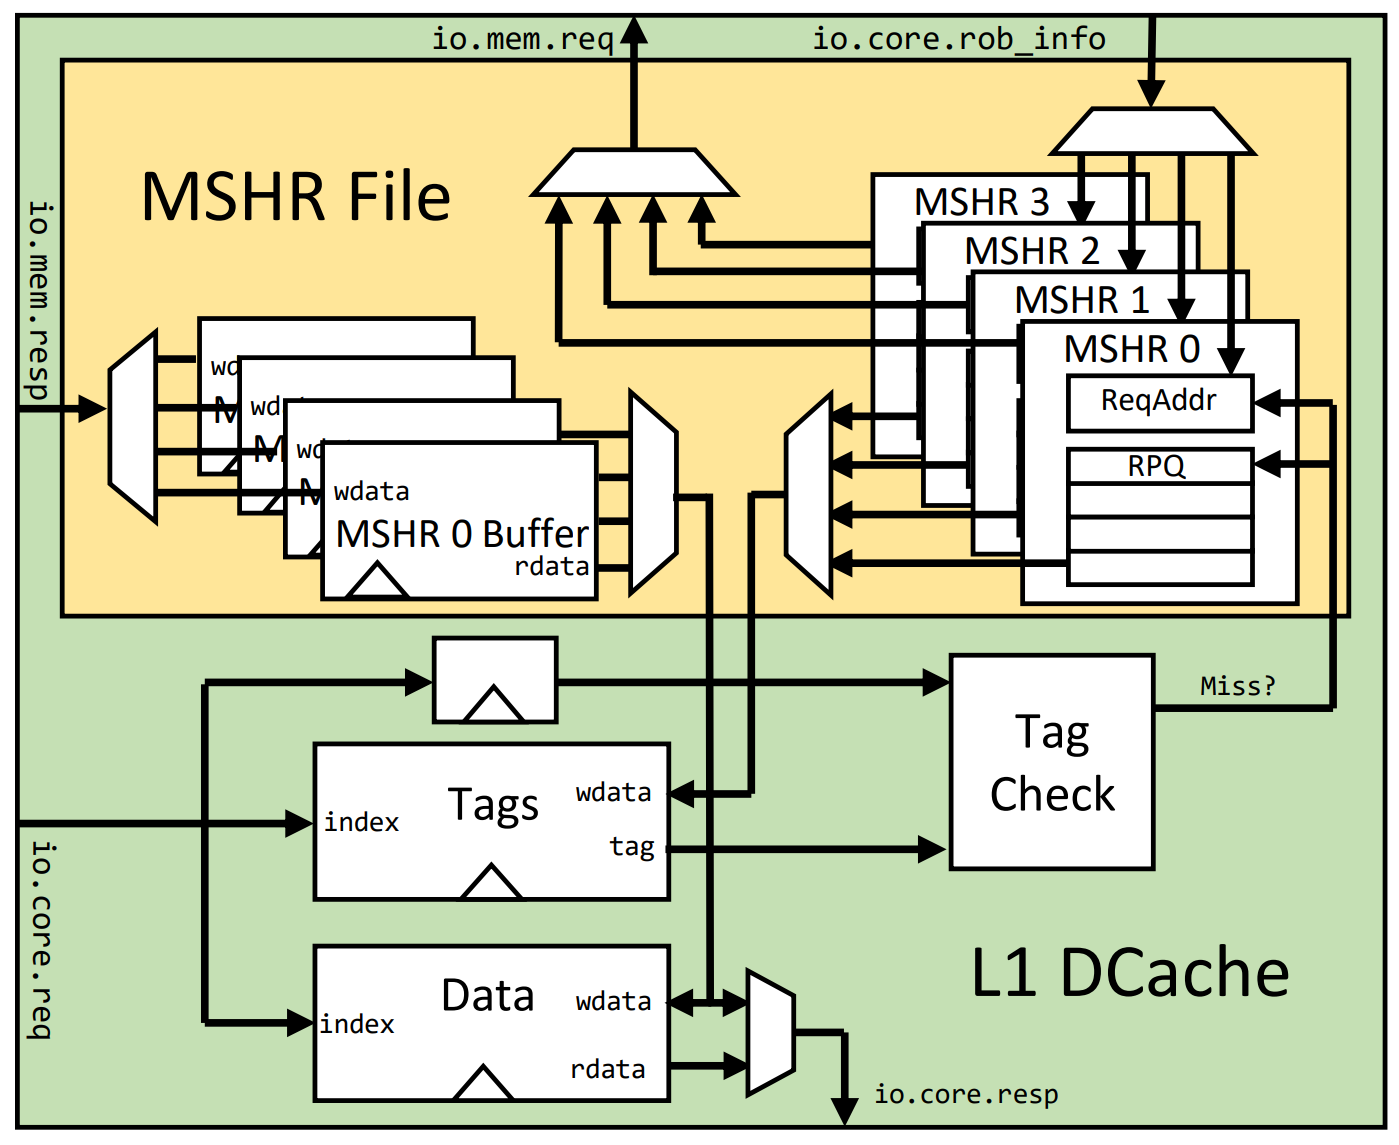
\includegraphics[scale=0.17]{dcache.png}\end{center}
  \caption{Overview of modified L1 data cache}
\end{figure}

\subsection{Point of No Return}
In the base implementation of the speculation buffer, entries in the buffer are only deallocated when the instruction is reached by the head of the reorder buffer (ROB). However, this can result in heavy MSHR utilization, as many instructions may reside between a waiting load and the commit head. However, we observe that many of those instructions, while still inflight, can be marked as guaranteed to commit.

This informs the concept of a ``point-of-no-return'' (PNR) in the ROB, in addition to the commit head. While the commit head tracks the next instruction which will commit the architectural state, the PNR tracks instructions which are guaranteed to eventually commit, even if they have not yet completed execution. In other words, the PNR points at the oldest instruction which may cause misspeculated execution; an unsafe instruction, such as a branch which has not yet executed. If an instruction is marked as safe, the PNR will pass it whether or not it has completed executing. We observe that refills in the spec-buffer can be committed to the cache as soon as the PNR passes the instruction which triggered them. This reduces pressure on MSHR resources and prevents backpressure on incoming cache requests.

To reduce the performance impacts of SpecBuf, we implemented a PNR in the ROB. Two versions were implemented. The first ``simple-PNR'' will only mark at most one ROB row per cycle as ``guaranteed to commit''. We also implemented a more complex ``fast-PNR'' that can mark an arbitrary number of rows per cycle, essentially ``jumping over'' groups of safe instructions to the oldest unsafe instruction. These are illustrated in figure~\ref{PNR}: the position of the PNR pointer on the subsequent cycle is shown for both the simple and fast versions.

\begin{figure}[h]
  \begin{center}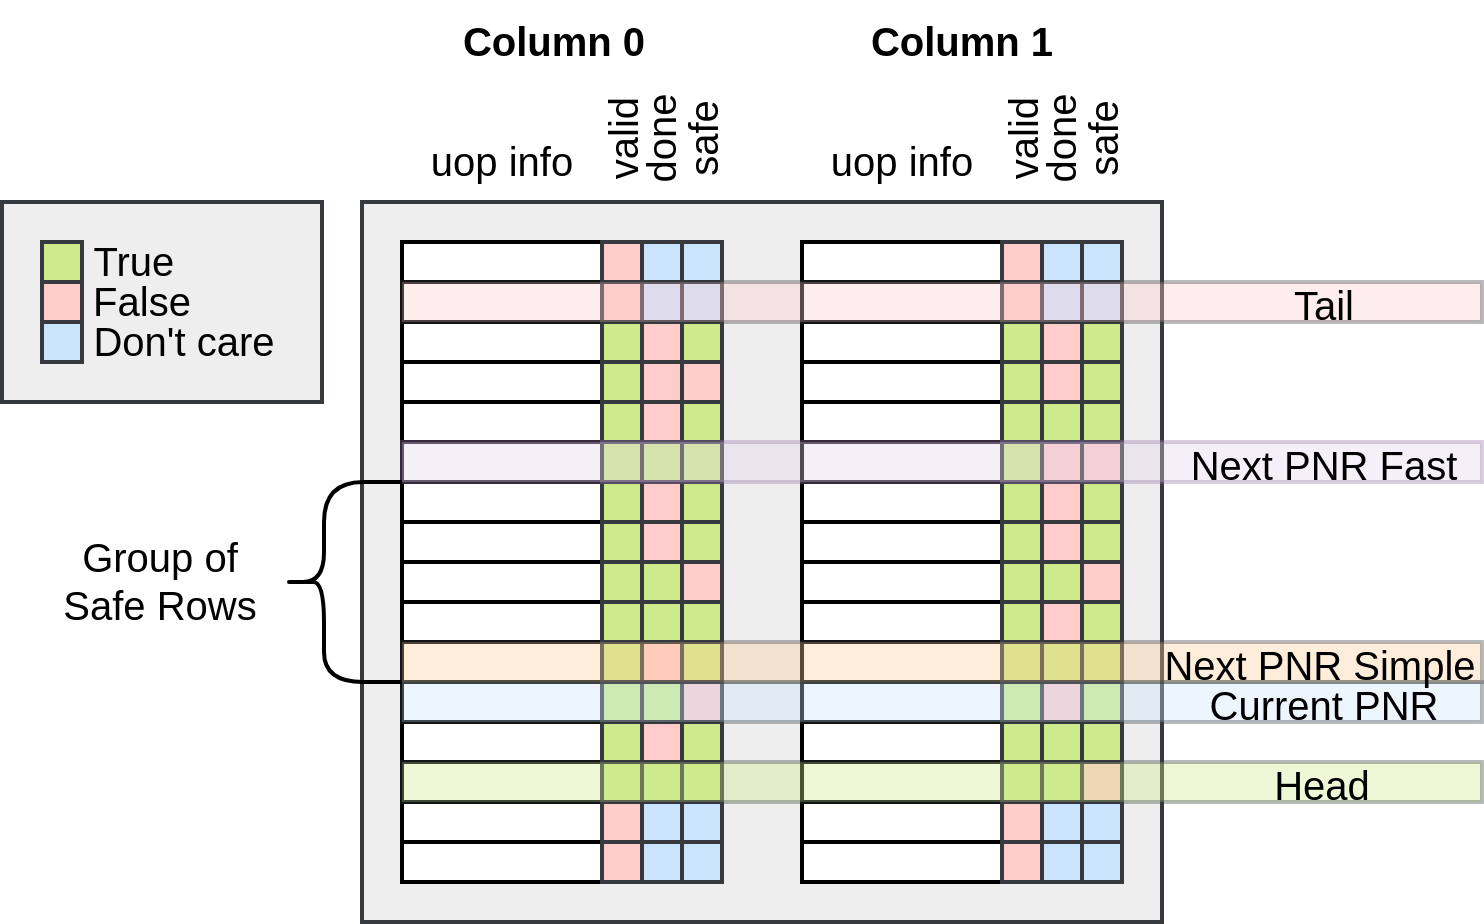
\includegraphics[scale=0.17]{rob_pnr.png}\end{center}
  \caption{Overview of PNR in ROB}
  \label{PNR}
\end{figure}

\subsection{Physical Optimization}
The speculative cache line buffers are by far the most physically costly addition to our secure boom variant. These buffers do not often need to be accessed simultaneously, and thus can be ``factored out'' of the MSHRs and into a single ported (1RW) or dual ported (1R/1W) SRAM. This would significantly decrease the (already modest \ref{syn}) area overhead incurred by these cache line buffers compared to when they are synthesized out of flip-flops.

\subsection{MSHR File as a Sidechannel}
A limitation which affects our current MSHR file implementation is that MSHRs are not always immediately deallocated after being killed. This limitation opens up several potential sidechannels which Spectre style attacks could use to extract information. For instance, when combined with the limitation of only allowing a single inflight miss to a particular cache set, the following attack surfaces: an attacker could perform their malicious call on a victim function repeatedly, following each call immediately with a single load which is known to miss, rather than an inspection of an entire attack array. If one of these loads took longer than expected of a miss, the attacker could deduce that a killed miss to the same set was being held by the MSHR, waiting for a response from the data bus. From this, the attacker infers part of the address used in the victim's secret-dependent load; 6 bits in a cache with 64 sets. This attack may be more difficult to perform than the standard attack, as there is a limited time window the MSHR will remain allocated following being killed. Additionally, this attack would be far slower as the victim call and probing sequence needs to be performed an average of $num\_sets/2$ times to read out $log_{2}(num\_sets)$ bits.

\subsubsection{Fully Associative MSHR File}
Making the MSHR file fully associative would aid in mitigating the side channel mentioned above. The number of MSHRs allocated could still be used as a side channel, however. The reason we have not made the MSHR file fully associative is the random replacement policy employed by the Rocket cache, which assumes only a single miss may be inflight per cache set. We would need to augment this policy with an index associative structure, with as many entries as there are MSHRs. This structure would track which ways of a particular set are scheduled to be replaced by an inflight miss. Note that this would not entirely mitigate the side channel, as the number of inflight misses to a particular set is now limited by the number of ways, as opposed to being singular. Thus, the attacker would need to simply perform more accesses.

\subsubsection{Immediately Killable MSHRs}
MSHRs are not immediately killable because they must acknowledge the L2 data bus when it has returned with the refill data. They must additionally forward out speculative loads which will be received and killed by the data cache shim; failure to forward out loads will result in a resource leak in this structure. To implement this functionality, we would need to implement a structure which tracks inflight refill requests. This structure would need to have more entries than the number of MSHRs; free entries would be mapped onto MSHRs upon a primary cache miss. Upon receiving a bus response, they would ``wake up'' their corresponding MSHR. Entries would be disassociated from MSHRs if the MSHR was killed early, and would be deallocated upon receiving and acknowledging their bus response. Additionally, we would be required to forward ``phony'' load responses to the data cache shim.

\section{Evaluations} \label{Evaluations}

\subsection{Base Core Parameters}

The two attacks were replicated on the BOOM core with the parameters given
in Table \ref{tab:boom-core-params}. All attacks were measured using FireSim, an open-source
cycle-accurate, FPGA-accelerated scale-out computer system simulation platform \cite{b12}.

\begin{table}
\centering \caption{BOOM Core Parameters} \label{tab:boom-core-params}
\begin{tabular}{@{} *2l @{}} \toprule
    Parameter                    & Value \\ \midrule
    Fetch Width                  & 2 \\
    Decode Width                 & 2 \\
    Issue Width                  & 4 \\
    PRF Size                     & 100 \\
    ROB Size                     & 100 \\ \midrule
    L1 Sets                      & 64 \\
    L1 Ways                      & 8 \\
    L1 Linesize                  & 64 bytes \\ \midrule
    BTB Sets                     & 512 \\
    BTB Banks                    & 2 \\
    BTB Ways                     & 4 \\ \midrule
    GShare History Bits          & 23 \\
    GShare Counter Table Entries & 4096 \\ \bottomrule
\end{tabular}
\end{table}

\begin{figure}
    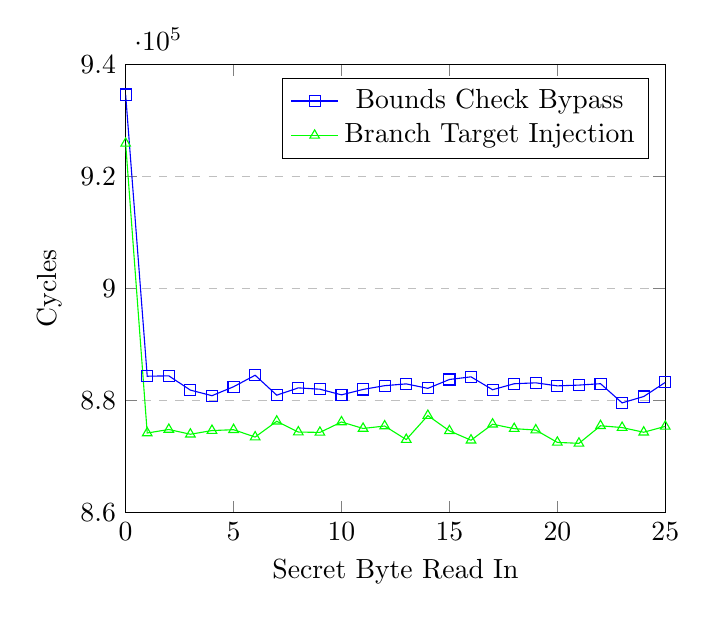
\begin{tikzpicture}
        \begin{axis}[
            ylabel={Cycles},
            xlabel={Secret Byte Read In},
            xmin=0, xmax=25,
            ymin=860000, ymax=940000,
            legend pos=north east,
            ymajorgrids=true,
            grid style=dashed
        ]
            \addplot[
                color=blue,
                mark=square,
            ]
            coordinates {
                (0 ,934580)
                (1 ,884322)
                (2 ,884387)
                (3 ,881845)
                (4 ,880847)
                (5 ,882446)
                (6 ,884498)
                (7 ,880939)
                (8 ,882241)
                (9 ,882006)
                (10,880994)
                (11,881965)
                (12,882634)
                (13,882954)
                (14,882156)
                (15,883738)
                (16,884212)
                (17,881912)
                (18,882980)
                (19,883142)
                (20,882600)
                (21,882739)
                (22,882989)
                (23,879563)
                (24,880698)
                (25,883218)
            };
                    
            \addplot[
                color=green,
                mark=triangle,
            ]
            coordinates {
                (0 ,925862)
                (1 ,874188)
                (2 ,874815)
                (3 ,873968)
                (4 ,874626)
                (5 ,874778)
                (6 ,873466)
                (7 ,876281)
                (8 ,874361)
                (9 ,874297)
                (10,876153)
                (11,875000)
                (12,875435)
                (13,873015)
                (14,877303)
                (15,874572)
                (16,872902)
                (17,875761)
                (18,874966)
                (19,874715)
                (20,872514)
                (21,872346)
                (22,875481)
                (23,875161)
                (24,874325)
                (25,875371)
            };
            \legend{Bounds Check Bypass,Branch Target Injection}
        \end{axis}
    \end{tikzpicture}
    \caption{Speed of Replicated Attacks}
    \label{fig:speed-attacks}
\end{figure}

\begin{lstlisting}[style=column-code, label={code:spec-attack-printout}, caption=Printout of Bounds Check Bypass Attack]
want(#) =?= 1.(#) 2.( C)
want(T) =?= 1.(T) 2.(^A)
want(h) =?= 1.(h) 2.(i)
want(i) =?= 1.(i) 2.(>)
want(s) =?= 1.(s) 2.(^D)
want(I) =?= 1.(I) 2.(^D)
want(s) =?= 1.(s) 2.( ^L)
want(T) =?= 1.(T) 2.( )
want(h) =?= 1.(h) 2.(^F)
want(e) =?= 1.(e) 2.()
want(B) =?= 1.(B) 2.(<9f>)
want(a) =?= 1.(a) 2.(^B)
want(b) =?= 1.(b) 2.(^A)
want(y) =?= 1.(y) 2.()
want(B) =?= 1.(B) 2.( )
want(o) =?= 1.(o) 2.(^H)
want(o) =?= 1.(o) 2.(4)
want(m) =?= 1.(m) 2.(k)
want(e) =?= 1.(e) 2.(^C)
want(r) =?= 1.(r) 2.(^A)
want(T) =?= 1.(T) 2.(^C)
want(e) =?= 1.(e) 2.(^O)
want(s) =?= 1.(s) 2.(^D)
want(t) =?= 1.(t) 2.(^A)
\end{lstlisting}

\subsection{Replicating Speculative Attacks Results}

Overall, the attacks chosen were replicated successfully on the BOOM microarchitecture. A printout
demonstrating leakage of secret information with the Bounds Check Bypass attack
is shown in Code \ref{code:spec-attack-printout}. Initial results of the replications
are promising with around 3.6KB/s for both attacks. Table \ref{tab:spec-attack-results}
shows the results of the two attacks while Figure \ref{fig:speed-attacks} shows the cycles per secret byte read out.
These measurements take into account the clearing
of the tally array before each run, the multiple rounds of training for the BPU,
the single attack run on the victim, and the time to measure out the secret from the attacker array.
The cycle times are close to each other because the code shares a similar structure. The main
differences are around the setup of the {\tt fdiv} manipulation
and the extra arithmetic in the Branch Target Injection attack where you have to calculate
both the index and the address for accessing the function and passing the input. 

\begin{table}
\centering
\caption{Attack Parameters}
\label{tab:attack-params}
\begin{tabular}{@{} *2l @{}} \toprule
    Parameter                    & Value \\ \midrule
    Cache Hit Threshold          & 50 cycles \\
    Amount of runs on same byte  & 10 rounds \\
    Training rounds for BPU      & 6 training rounds \\
    Cache flush hits on same set & 4 * L1\_WAYS \\
    GShare Counter Table Entries & 4096 \\ \bottomrule
\end{tabular}
\end{table} 

\begin{table}
\centering
\caption{Speculative Attack Results}
\label{tab:spec-attack-results}
\begin{tabular}{@{} *4l @{}} \toprule
    &                        & \multicolumn{2}{l}{Bytes per Second} \\
    Attack                  & Cycles for Secret Byte &           100 MHz &   3.2 GHz \\ \midrule
    Bounds Check Bypass     &                ~884485 &          ~113 B/s & ~3618 B/s \\
    Branch Target Injection &                ~876602 &          ~114 B/s & ~3650 B/s \\ \bottomrule
\end{tabular}
\end{table}

\subsection{SpecBuf Results}

We evaluated our SpecBuf implementation using three small microbenchmarks, Dhrystone and the 
replicated attacks. The microbenchmarks created stress the MSHR blocking and eviction conditions
that slow down the machine while Dhrystone was chosen as an initial general test. The SpecBuf shows an expected small decrease
in performance in the microbenchmark tests while Dhrystone shows a small improvement all while providing
a defense against the replicated attacks demonstrated. A table of results is shown at Table \ref{tab:spec-buf-results}.

\subsubsection{Microbenchmark Explanations and Results}

The first microbenchmark named "Non-speculative load misses to same sets" was used to test how efficient non-speculative loads
were when the MSHR was unable to allocated entries for each new load. This microbenchmark is a series of loads that had different
tags but the same index, thus in BOOM's MSHR, only one entry would be able to be allocated at a time. When using the SpecBuf, the 
behavior is similar. The main difference is that on each load, the data from cache hierarchy must first fill the MSHR buffer
before the cache. This causes a small performance decrease for each load. Since our benchmark has 16 loads, this results in a performance decrease of around
{\tt 16 loads * (CACHE\_LINE\_SZ / DATABUS\_WIDTH)} or {\tt 16 * (64B / 8B) = 128 cycles}.

The second microbenchmark named "Non-speculative load misses to different sets" is similar to the first except that each subsequent
load is accessing a different set in the cache. In the normal version of BOOM, the MSHR's would fill up completely but then stall 
when full until a prior MSHR entry would be freed (when a previous load is completed). When using the SpecBuf, there is a
higher performance penalty because the data must fill the MSHR buffer with the cache data before filling the cache. Thus, there 
is a extra overhead of around 8 cycles for every 4 loads since the MSHR's are allocated waves of 4 and the fill latency to the MSHR
buffer is {\tt CACHE\_LINE\_SZ / DATABUS\_WIDTH} or {\tt 64B / 8B = 8 cycles}.

The final microbenchmark named "MSHR evicted speculative load miss" is used to test the impact when a load has to be evicted from the 
MSHR due to a potential deadlock condition. In the normal version of BOOM, if a speculative load is issued to the 
MSHR before a critical load that resolves the speculation, the speculative load will complete and
write it's data to the cache. This will release the MSHR entry it occupied and allow the critical load to complete resolving the speculation. 
However, the SpecBuf case, the speculative load will fill the data in the MSHR buffer, bypass the data to the microarchitectural register, 
then wait for speculation to finish to determine if the data will go into the cache. If the critical load that needs the MSHR is issued after the speculative load,
then the speculative load is evicted from the data cache resulting the data from that MSHR entry not entering the data cache. If the 
flow was speculated to be correct, then any following loads that have the same set and tag would miss in the cache causing a performance decrease.
This microbenchmark shows this performance hit on the first load that occurs after this case.

\subsubsection{Dhrystone Results}
Enabling the SpecBuf granted a 2\% increase in Dhrystone performance, seen below in Table \ref{tab:spec-buf-results}. There are several factors which may contribute to this small performance gain. The SpecBuf delays the eviction of old cachelines until the refill is known to commit, allowing hits on the old cacheline in the intervening cycles. Additionally, the SpecBuf decreases the latency of missed loads: this is because refill requests can be sent to the bus earlier, and the retured data can be forwarded out of the buffer as soon as it is available, rather than waiting for the update of cache metadata.

\begin{table}
\centering
\caption{SpecBuf Results}
\label{tab:spec-buf-results}
\begin{tabular}{@{} *4l @{}} \toprule
    & \multicolumn{2}{l}{Version of BOOM} & \\
    Benchmark                           & Normal & SpecBuf & \% Diff.\\ \midrule
    Non-spec. LD misses   & 540 cycles & 640 cycles & -19\%    \\
    to same sets            &            &            & \\ \midrule
    Non-spec. LD misses   & 264 cycles & 297 cycles & -11\%    \\ 
    to diff. sets           &            &            & \\ \midrule
    MSHR evicted spec. & 48 cycles & 67 cycles & -40\%    \\
    LD miss                &            &            & \\ \midrule
    Dhrystone                           & 2176 Dhrystones/s & 2216 Dhrystones/s & +2\%\\ \bottomrule
\end{tabular}
\end{table}

\subsubsection{Synthesis Results} \label{Synthesis Results}
Trial synthesis of BOOM with our SpecBuf in a 45nm technology resulted in a 2.5\% increase in area and a 0.36\% decrease in clock frequency using HAMMER, a framework to
abstract synthesis and place-and-route \cite{hammer}.



\section{Future Work}

\subsection{Bounds Check Bypass and Branch Target Injection Improvements}

While the replicated attacks are a PoC of a subset of speculative style attacks that BOOM
is susceptible to, future work can improve the secret leakage rate of the attacks.

One of the mechanisms to speed up both attacks is the improving the hand-made L1 cache line flush function
used. The current implementation uses a large extra array that is indexed into to evict a particular
cache set. Another approach, would be to just have this extra array be the size of the L1 cache and use
arithmetic to figure out which entry to index into to evict the requested cache line. This decreases the
amount of extra memory needed to run the function while allowing the statically allocated array to reside
at any memory location. Additionally, another approach to speeding up the function is to know where the
secret and probed array reside in memory. This allows the function to predetermine which addresses can be 
accessed to evict any particular line in the cache instead of doing arithmetic to index into the extra array and
having multiple branches that may misspeculate.

In addition to improving the cache line flush function, another
improvement can be to tweak the different attack parameters. This includes
the attack parameters listed in \ref{tab:attack-params}. Potentially, the amount of rounds on the
same byte and training rounds can be reduced to improve the speed of the attack.
These can be adjusted in conjunction with the cache flush hits on the same set so even though the 
random cache replacement policy may not clear all the ways of the set, the amount of rounds on
the same byte might remove the false hits when the specified line was not evicted.

\subsection{Other Attacks and More BOOM Configurations}

In addition to the two attacks that were implemented, BOOM is susceptible to a variety of
other speculative style attacks. One such example is the RSB attack, which our team was 
originally planning on implementing. However, due to BOOM not have a working configuration
with the RSB at the time, this attack was not implemented in liew of implementing the Branch Target
Injection attack. By fixing the RSB, the team could work on implementing this attack with the 
code that was initially created for it. Another improvement to the project would be to train the
variety of attacks on different branch predictors. Since BOOM provides a mechanism to add branch 
predictors and it already has a TAGE predictor, future work can use this functionality to determine
the speed of the attacks based these new predictors.

\subsection{Further Evaluations}

We plan to perform a more through evaluation of the performance and security implications of the
speculation buffer after more validation on our design is complete. 
Though the Dhrystone benchmark was able to be run, a more comphrehensive benchmark suite would be invaluable to test
the performance of the SpecBuf. At evaluation, the SpecBuf was unable to boot RISC-V Linux on FireSim and therefore
we were unable to run the SPEC2017 suite \cite{b50}. Additionally, the SpecBuf was unable to run the CoreMark EEMBC benchmark
suite due to bugs that occured 5M cycles into the suite \cite{b51}. Thus, future work would be to fix the bugs preventing these
benchmarks to run and reevaluate the results of the paper based on this new data. We also plan to configure multiple design
points of the speculation buffer with multiple implementations of the PnR head and refill/replay system.

Get better synthesis data from HAMMER \cite{b52}. Instead of using flops use sram to have a minimal 
physical impact.

\subsection{BOOM Improvements}

Future work for the project also involves bringing BOOM to a more stable version. Throughout
the project, a multitude of performance-reducing bugs were found both in the front-end (fetch stage, BPU, etc) and the 
load/store unit that the team had to work around. With these fixed, not only will performance
of the core improve, but other replication and modifications to the core will be easier since
the base core will be stable and provide more reliable performance metrics.

\subsubsection{Multiported Cache}
The non-blocking L1 data cache employed in BOOM was designed with the in-order Rocket core in mind; is not ideal for
a high performance out-of-order core. This is for several reasons.

Firstly the cache does not have any concept of speculative execution.
In the baseline version of BOOM, this is bridged with an external ``data cache shim'' stucture. We have further introduced the cache to the
concept of speculative execution by propagating the necessary signals through the first two stages and into the MSHR file.

Second, the cache contains many structures and provisions which are superfluous in an out-of-order core.
For instance, the job of the replay queues would be better handled by the core's load/store unit itself.

Finally, the cache is strictly single ported. In order to investigate high performance variants of the BOOM core,
a multiported data cache will be required.

\subsubsection{Speculation Buffer Improvements}
Our current speculation buffer implementation has several limitations, mentioned in \ref{specbuf}.
Among them are the lack of full-associativity, the inability to immediately deallocate killed MSHRs, and MSHR state sequences which are not fully optimized.
We may be able to implement some of these improvements in our proof-of-concept speculation buffer, but others would be more difficult. To improve further upon
our proof-of-concept, we may be better served by looking at re-architecting BOOM's data cache with speculative safety in mind. This builds upon our other thoughts
on BOOM's data cache mentioned above.

\subsubsection{Multi-level Cache Hierarchy}
The current speculation buffer addresses only a single level cache hierarchy.
BOOM is currently configured with an L1 data cache and a large scratchpad memory.
In the future, it would be valuable to configure BOOM with a more realistic cache hierarchy,
such as with a large L2 shared between several cores. This would lend towards an extension of the speculation
buffer strategy to protect this realistic hierarchy.

\section{Conclusion}


\begin{thebibliography}{00}
    \bibitem{b1} P. Kocher, D. Genkin, D. Gruss, W. Haas, M. Hamburg, M. Lipp, S. Mangard, T. Prescher, M. Schwarz, and Y. Yarom, ``Spectre attacks: Exploiting speculative execution,'' ArXiv e-prints, Jan. 2018
    \bibitem{b2} M. Lipp, M. Schwarz, D. Gruss, T. Prescher, W. Haas, A. Fogh, J. Horn, S. Mangard, P. Kocher, D. Genkin, Y. Yarom, M. Hamburg, ``Meltdown: Reading Kernel Memory from User Space,'' 27th USENIX Security Symposium, 2018
    \bibitem{b3} E. M. Koruyeh, K. N. Khasawneh, C. Song, N. Abu-Ghazaleh, ``Spectre Returns! Speculation Attacks using the Return Stack Buffer,'' 12th USENIX Workshop on Offensive Technologies, 2018
    \bibitem{b4} G. Maisuradze, C. Rossow, ``ret2spec: Speculative Execution Using Return Stack Buffers,'' 25th ACM Conference on Computer and Communications Security, 2018
    \bibitem{b5} J. Renau, ``Securing SoCs from Time Side Channels,'' UC Santa Cruz, 2018
    \bibitem{b6} G. Irazoqui, X. Guo, ``Cache Side Channel Attack: Exploitability and Countermeasures,'' Black Hat Asia, 2017
    \bibitem{b7} J. Schmidt, ``Exclusive: Spectre-NG - Multiple new Intel CPU flaws revealed, several serious,'' Heise.de, 2018
    \bibitem{b8} V. Kiriansky, I. Lebedev, S. Amarasinghe, S. Devadas, J. Emer, ``DAWG: A Defense Against Cache Timing Attacks in Speculative Execution Processors,'' MICRO, 2018
    \bibitem{b9} R. Spreitzer, V. Moonsamy, T. Korak, S. Mangard, ``Systematic classification of side-channel attacks: a case study for mobile devices,'' CoRR, 2018
    \bibitem{b10} Q. Ge, Y. Yarom, D. Cock, G. Heise, ``A Survey of Microarchitectural Timing Attacks and Countermeasures on Contemporary Hardware'', IACR, 2016
    \bibitem{b11} C. Celio, D. A. Patterson, K. Asanović, ``The Berkeley Out-of-Order Machine (BOOM): An Industry-Competitive, Synthesizable, Parameterized RISC-V Processor,'' Technical Report, June 2015
    \bibitem{b12} S. Karandikar, H. Mao, D. Kim, D. Biancolin, A. Amid, D. Lee, N. Pemberton, E. Amaro, C. Schmidt, A. Chopra, Q. Huang, K. Kovacs, B. Nikolic, R. Katz, J. Bachrach, and K. Asanović, ``FireSim: FPGA-Accelerated Cycle-Exact Scale-Out System Simulation in the Public Cloud,'' ISCA, 2018
\end{thebibliography}


\newpage
%\vspace{20em}
%\afterpage{\clearpage}
\section*{Appendix A\\
          Bounds Check Bypass BOOM Proof of Concept}

In Code \ref{code:boom-spectre-v1} is the implementation of the Bound Check Bypass attack
on BOOM. Without speculation, the {\tt array2} access in the {\tt victimFunc} would be only accessed
during the training round with the value retrieved from {\tt array1}. However, since speculation occurs, the {\tt array2} is accessed with
the secret value during the attacker run by having {\tt array1} be used to reach the {\tt secretString} value.

\onecolumn
\lstinputlisting[style=full-code, label={code:boom-spectre-v1}, caption=BOOM Proof of Concept code of Bounds Check Bypass Attack]{condBranchMispred.c}


\end{document}
